\section{SYSTEM DESIGN (Engineering Thinking)}
Hệ thống được thiết kế dựa trên nguyên lý \textbf{Decomposition} (Phân rã hệ thống) và \textbf{Abstraction} (Trừu tượng hóa dữ liệu), chia nhỏ một bài toán học tập ngôn ngữ phức tạp thành các module phần mềm độc lập nhưng giao tiếp chặt chẽ với nhau trên môi trường cục bộ (Local). 
\subsection{Overall Architecture (Kiến trúc tổng thể)}
Vì game chạy 100\% local, kiến trúc hệ thống sẽ là một ứng dụng Desktop nguyên khối (Monolithic Desktop App) giao tiếp với các dịch vụ cục bộ. \newline
\textbf{Sơ đồ C4 (gồm C1: context và C2: container):}
\begin{figure}[H]
	\centering
	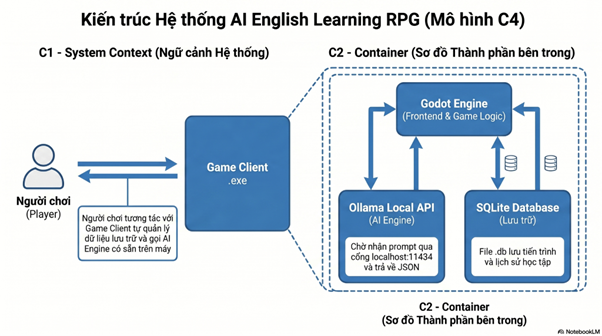
\includegraphics[scale=1]{Figure/mohinhc4.png}
	\caption{Sơ đồ C4}
	\label{fig:sodoc4}
\end{figure}

\subsection{Module Design}
Hệ thống được chia thành 4 module chính:
\begin{enumerate}
	\item \textbf{UI/UX Module (Godot):}
	\begin{itemize}
		\item \textit{Scene Manager:} Quản lý luồng hiển thị giữa Bản đồ thế giới và Màn hình chiến đấu. 
		\item \textit{Real-time Evaluation UI:} Hiển thị câu hỏi, nút đáp án và giao diện xuất hiện của NPC AI kèm lời giải thích.
	\end{itemize}
	\item \textbf{Core Game Logic (Godot):}
	\begin{itemize}
		\item \textit{Asynchronous Pre-generation Engine:} Chạy ngầm (background thread). Âm thầm truy vấn SQLite và gọi API Ollama khi người chơi đang di chuyển trên bản đồ, lưu kết quả vào Cache để loại bỏ hoàn toàn độ trễ khi vào trận đấu.
		\item \textit{Hierarchical Competency Gating:} Giám sát tiến độ tiêu diệt quái vật để mở khóa các phân vùng từ vựng khó hơn (Tier 1, Tier 2).
	\end{itemize}
	
	\item \textbf{AI Integration Module (Godot + Ollama):}
	\begin{itemize}
		\item \textit{Context-Aware Prompt Builder:} Dựa vào thông số loại quái vật và môi trường xung quanh (Biome) để chèn vào System Prompt, gửi tới AI để sinh đề bài khớp ngữ cảnh.
		\item \textit{JSON Parser:} Bóc tách dữ liệu phản hồi từ AI lấy cấu trúc câu hỏi, đáp án, và phần giải thích (Explainable AI).
	\end{itemize}
	
	\item \textbf{Data Tracking Module (SQLite):}
	\begin{itemize}
		\item \textit{Knowledge Tracing System:} Lưu trữ tỷ lệ trả lời đúng/sai của người chơi trên từng từ vựng cụ thể. 
	\end{itemize}
\end{enumerate}

\subsection{CT System Mapping (Traceability)}
Bảng ánh xạ dưới đây thể hiện cách các trụ cột của Tư duy tính toán định hình nên kiến trúc hệ thống: 

\begin{table}[H]
\centering
\caption{Ma trận liên kết Trụ cột Tư duy tính toán và Thành phần Hệ thống}
\label{tab:ct_framework_matrix}
\small
\noindent\begin{tabularx}{\textwidth}{|>{\raggedright\arraybackslash}p{2.8cm}|X|>{\raggedright\arraybackslash}p{3.2cm}|>{\raggedright\arraybackslash}p{2.2cm}|}
\hline
\textbf{CT Pillar (Trụ cột TDTT)} & \textbf{Mạch Logic (Business Logic)} & \textbf{System Component (Thành phần hệ thống)} & \textbf{Liên kết Core Feature} \\ \hline

\textbf{Decomposition} \newline (Phân rã bài toán) & 
Chia nhỏ toàn bộ dữ liệu từ vựng khổng lồ thành các mảnh dữ liệu nhỏ, gắn chặt với từng phân cấp quái vật và khu vực cụ thể trên Map. & 
Hierarchical Gating Controller (Godot) \& Data Partitioning (SQLite) & 
Feature 5 \\ \hline

\textbf{Pattern Recognition} \newline (Nhận diện mẫu) & 
Theo dõi và nhận diện các mẫu lỗi sai (\textit{pattern of mistakes}) lặp lại thường xuyên của người chơi trong lúc làm bài để định lượng điểm yếu. & 
Knowledge Tracing System (SQLite Database) & 
Feature 3 \\ \hline

\textbf{Abstraction} \newline (Trừu tượng hóa) & 
Lọc bỏ các chi tiết thừa, biến đổi bối cảnh phức tạp của game (biome, loại quái, level) thành các tham số cốt lõi để ghép thành Prompt giao tiếp với AI. & 
Context-Aware Prompt Builder (Godot) & 
Feature 4 \\ \hline

\textbf{Algorithm Design} \newline (Thiết kế thuật toán) & 
Xây dựng luồng xử lý bất đồng bộ (chạy ngầm) để sinh đề/chấm điểm và thuật toán điều chỉnh độ khó động (DDA) dựa trên trình độ người chơi. & 
Async Pre-generation Engine (Godot) + Ollama Local API & 
Feature 1, 2 \& 6 \\ \hline
\end{tabularx}
\end{table}

\subsection{Data Flow (Luồng dữ liệu)}
\textbf{Sơ đồ luồng dữ liệu (Data Flow Diagram - DFD) dạng khối hình học (Flowchart diagram):}
\begin{figure}[H]
	\centering
	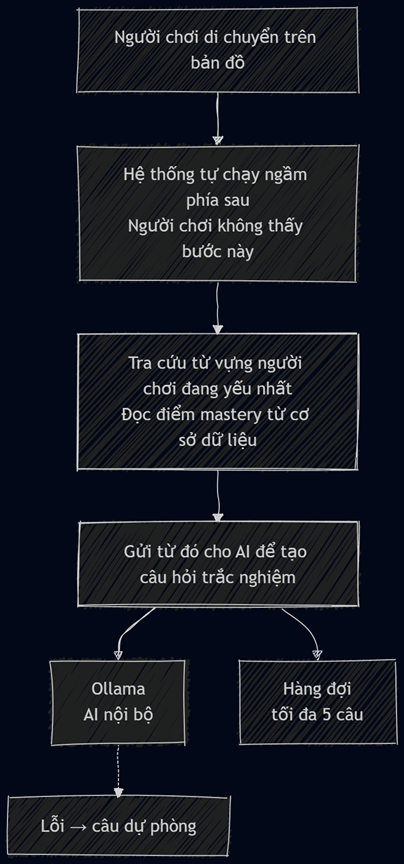
\includegraphics[scale=1]{Figure/df1.png}
	\label{fig:df1}
\end{figure}

\begin{figure}[H]
	\centering
	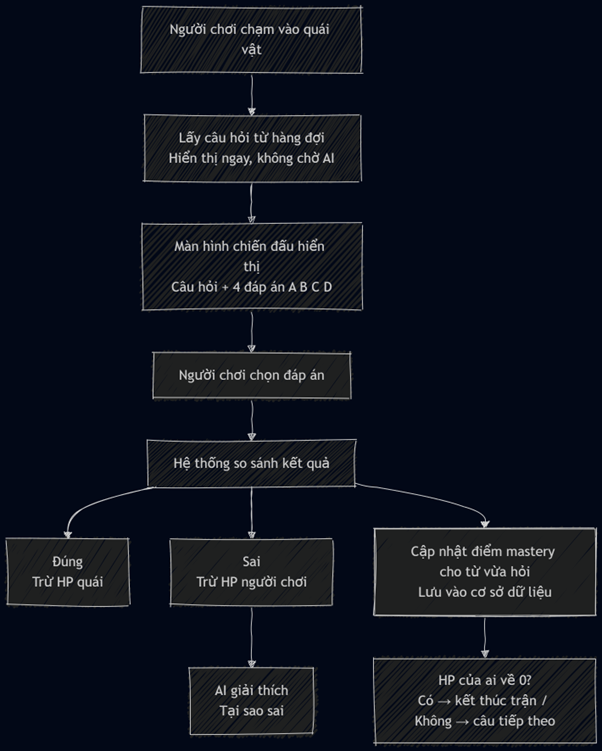
\includegraphics[scale=1]{Figure/df2.png}
	\label{fig:df2}
\end{figure}

\subsection{Use Case / Sequence Diagram}
\subsubsection{Use Cases}

\begin{description}
    \item[Use Case 1: Bắt đầu hoặc tiếp tục hành trình] \hfill
    \begin{description}
        \item[Tên Use Case:] Khởi tạo / Tải tiến trình game
        \item[Mục tiêu:] Cho phép người chơi bắt đầu một hành trình học từ vựng mới hoặc tiếp tục từ lần chơi trước.
        \item[Tác nhân:] Người chơi, Cơ sở dữ liệu SQLite
        \item[Điều kiện tiên quyết:] Người chơi đã mở file game thành công trên máy tính.
        \item[Hậu điều kiện:] Màn hình bản đồ hiển thị, nhân vật sẵn sàng di chuyển.
        \item[Các bước thực hiện:] \hfill
        \begin{enumerate}
            \item Hệ thống hiển thị màn hình chính với hai lựa chọn: \texttt{New Game} và \texttt{Continue}.
            \item Nếu người chơi chọn \texttt{New Game}: hệ thống tạo hồ sơ mới (HP đầy, điểm mastery về mức ban đầu) và đưa người chơi vào Chapter 1.
            \item Nếu người chơi chọn \texttt{Continue}: hệ thống đọc file \texttt{save.db} để khôi phục vị trí trên bản đồ, HP, và lịch sử học từ vựng.
            \item Hệ thống tải tài nguyên game và đặt nhân vật đúng vị trí đã lưu.
        \end{enumerate}
        \item[Kịch bản phụ:] Nếu file lưu bị mất hoặc hỏng, hệ thống ẩn nút \texttt{Continue}, hiển thị thông báo ``Không tìm thấy dữ liệu lưu'' và yêu cầu người chơi chọn \texttt{New Game}.
    \end{description}

    \vspace{0.3cm} % Tạo khoảng cách nhỏ giữa các Use Case

    \item[Use Case 2: Khám phá bản đồ] \hfill
    \begin{description}
        \item[Tên Use Case:] Di chuyển và khám phá thế giới game
        \item[Mục tiêu:] Người chơi di chuyển tự do trên bản đồ, trong khi hệ thống tự động chuẩn bị sẵn câu hỏi cho trận chiến tiếp theo.
        \item[Tác nhân:] Người chơi, Ollama (AI chạy trên máy người chơi)
        \item[Điều kiện tiên quyết:] Người chơi đang ở màn hình bản đồ thế giới.
        \item[Hậu điều kiện:] Luôn có sẵn tối đa 5 câu hỏi trong bộ nhớ đệm, sẵn sàng cho trận chiến bất cứ lúc nào.
        \item[Các bước thực hiện:] \hfill
        \begin{enumerate}
            \item Người chơi dùng phím \texttt{WASD} để di chuyển nhân vật trên bản đồ.
            \item Song song với việc người chơi di chuyển, hệ thống âm thầm chạy ngầm phía sau.
            \item Hệ thống tra cứu danh sách từ vựng mà người chơi đang yếu nhất trong tier hiện tại.
            \item Hệ thống gửi yêu cầu đến Ollama để tạo câu hỏi trắc nghiệm phù hợp với trình độ.
            \item Câu hỏi được tạo xong sẽ được lưu vào hàng đợi bộ nhớ, không hiển thị ngay cho người chơi.
        \end{enumerate}
        \item[Kịch bản phụ:] Nếu Ollama phản hồi lỗi hoặc quá chậm, hệ thống tự động điền câu hỏi dự phòng có sẵn vào hàng đợi để game không bị gián đoạn. Sau 2 giây, hệ thống tự thử kết nối lại Ollama mà không cần người chơi can thiệp.
    \end{description}

    \vspace{0.3cm}

    \item[Use Case 3: Chạm trán quái vật] \hfill
    \begin{description}
        \item[Tên Use Case:] Tiếp cận và kích hoạt trận chiến
        \item[Mục tiêu:] Kiểm tra xem người chơi có đủ điều kiện để thách đấu loại quái vật hiện tại không, sau đó chuyển sang màn hình chiến đấu.
        \item[Tác nhân:] Người chơi
        \item[Điều kiện tiên quyết:] Người chơi đang di chuyển trên bản đồ và tiếp cận một quái vật.
        \item[Hậu điều kiện:] Màn hình chuyển sang giao diện chiến đấu, hoặc người chơi được yêu cầu luyện tập thêm với quái cấp thấp hơn.
        \item[Các bước thực hiện:] \hfill
        \begin{enumerate}
            \item Người chơi di chuyển nhân vật đến gần và chạm vào quái vật.
            \item Hệ thống đọc cấp độ (tier) của quái vật --- ví dụ: Slime thuộc Tier 1, Goblin thuộc Tier 2.
            \item Hệ thống kiểm tra tiến trình của người chơi xem đã đáp ứng điều kiện mở khóa quái vật này chưa.
            \item Nếu đủ điều kiện, màn hình chuyển cảnh sang giao diện chiến đấu.
        \end{enumerate}
        \item[Kịch bản phụ:] Nếu người chơi chưa đủ điều kiện (ví dụ: cố tấn công Goblin khi chưa chinh phục đủ Slime), hệ thống hiển thị hộp thoại: ``Vốn từ vựng của bạn chưa đủ để vào khu vực này. Hãy luyện tập thêm với quái vật ở khu vực trước!'' và giữ nguyên màn hình bản đồ.
    \end{description}

    \vspace{0.3cm}

    \item[Use Case 4: Chiến đấu trắc nghiệm] \hfill
    \begin{description}
        \item[Tên Use Case:] Trả lời câu hỏi để chiến đấu
        \item[Mục tiêu:] Người chơi trả lời câu hỏi trắc nghiệm từ vựng tiếng Anh để tấn công quái vật, đồng thời nhận giải thích tức thì từ AI khi trả lời sai.
        \item[Tác nhân:] Người chơi
        \item[Điều kiện tiên quyết:] Người chơi đã vào màn hình chiến đấu và hàng đợi câu hỏi đã có sẵn dữ liệu.
        \item[Hậu điều kiện:] Kết thúc trận chiến, điểm mastery của từ vựng liên quan được cập nhật vào cơ sở dữ liệu.
        \item[Các bước thực hiện:] \hfill
        \begin{enumerate}
            \item Hệ thống hiển thị câu hỏi trắc nghiệm kèm 4 đáp án A, B, C, D.
            \item Người chơi đọc câu hỏi và chọn một đáp án bằng cách click.
            \item Hệ thống đối chiếu đáp án của người chơi với đáp án đúng.
            \item Nếu đúng: nhân vật tấn công quái vật, trừ HP quái.
            \item Nếu sai: quái vật phản công, trừ HP người chơi. Hệ thống hiển thị bảng giải thích của AI nêu rõ tại sao đáp án đó sai.
            \item Hệ thống ghi lại kết quả vào hồ sơ từ vựng, cập nhật điểm mastery của từ vừa xuất hiện.
            \item Vòng lặp tiếp tục với câu hỏi mới cho đến khi HP của quái vật hoặc của người chơi về 0.
        \end{enumerate}
        \item[Kịch bản phụ:] Nếu câu hỏi lấy từ hàng đợi bị lỗi định dạng, hệ thống tự động bỏ qua câu đó và lấy câu tiếp theo ngay lập tức, người chơi không nhận ra sự gián đoạn. Nếu hàng đợi hoàn toàn trống, hệ thống sử dụng câu hỏi dự phòng có sẵn (\texttt{word\_id = -1}) và không ghi kết quả vào cơ sở dữ liệu để tránh dữ liệu rác.
    \end{description}

    \vspace{0.3cm}

    \item[Use Case 5: Xem sổ tay từ vựng] \hfill
    \begin{description}
        \item[Tên Use Case:] Tra cứu và ôn tập từ vựng đã học
        \item[Mục tiêu:] Người chơi xem lại toàn bộ từ vựng đã gặp trong game, biết từ nào mình đang yếu để chủ động ôn tập.
        \item[Tác nhân:] Người chơi
        \item[Điều kiện tiên quyết:] Người chơi đang ở màn hình bản đồ, không trong trạng thái chiến đấu.
        \item[Hậu điều kiện:] Người chơi đóng sổ tay và tiếp tục điều khiển nhân vật bình thường.
        \item[Các bước thực hiện:] \hfill
        \begin{enumerate}
            \item Người chơi nhấn phím \texttt{E} hoặc click vào biểu tượng quyển sách trên màn hình.
            \item Hệ thống truy vấn dữ liệu học tập của người chơi từ cơ sở dữ liệu.
            \item Giao diện sổ tay hiển thị danh sách từ vựng đã gặp, phân loại bằng màu sắc: đỏ là từ hay sai, xanh lá là từ đã thành thạo.
            \item Người chơi click vào một từ bất kỳ để xem nghĩa, ví dụ sử dụng và gợi ý ôn tập.
            \item Người chơi click nút Thoát để đóng sổ tay và quay lại game.
        \end{enumerate}
        \item[Kịch bản phụ:] Nếu người chơi chưa gặp từ vựng nào (ví dụ mới bắt đầu game), sổ tay hiển thị thông báo ``Bạn chưa gặp từ vựng nào. Hãy bắt đầu khám phá!'' thay vì danh sách trống.
    \end{description}
\end{description}

\subsubsection{Sequence Diagram}
\begin{figure}[H]
	\centering
	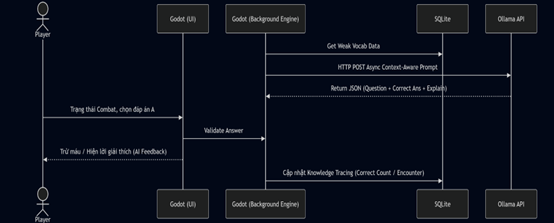
\includegraphics[scale=1.25]{Figure/SD.png}
	\label{fig:sd}
\end{figure}

\subsection{Data Design \& Modeling (Thiết kế Dữ liệu - Table Schema)}
\textbf{Table schema/ERD:}
\begin{figure}[H]
	\centering
	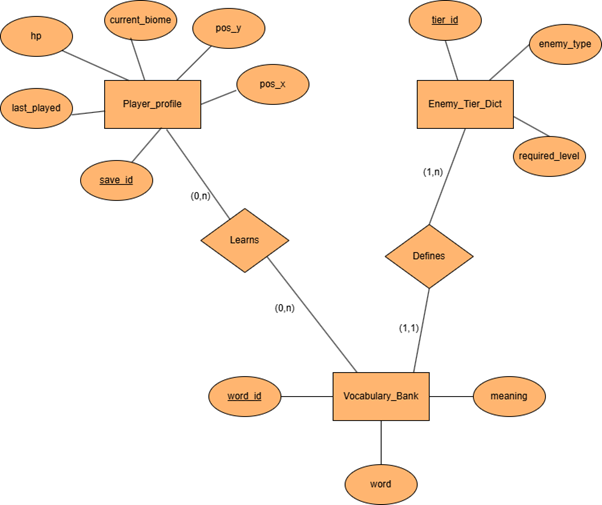
\includegraphics[scale=1]{Figure/erd.png}
	\label{fig:erd}
\end{figure}

\subsection{UI/UX Design \& Interactive Prototype (Figma) DTP}
\subsubsection{Design Concept \& Style Guide}
\subsubsection{High-Fidelity Mockups}
Dựa trên luồng trải nghiệm thực tế của người chơi, các giao diện được thiết kế và sắp xếp theo trình tự sau: 	
\begin{itemize}
	\item \textbf{Màn hình chính:} Điểm chạm đầu tiên của người chơi. Gồm logo tên game ở vị trí trung tâm với phông nền là ảnh sơ bộ của hòn đảo đầu tiên góc nhìn từ trên xuống. Bao gồm các nút điều hướng cơ bản: \textit{New game (bắt đầu)}, \textit{continue (chơi tiếp)}, \textit{options (cài đặt)} và \textit{quit game (thoát)}. 
	\begin{figure}[H]
	\centering
	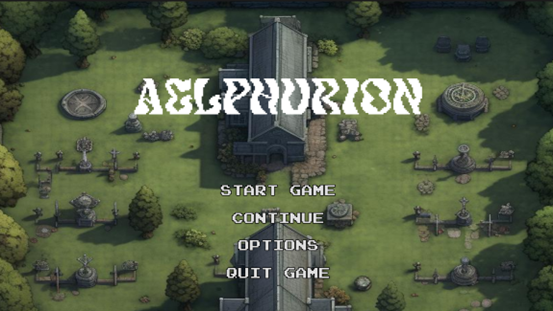
\includegraphics[scale=0.7]{Figure/titlescreen.png}
	\label{fig:title}
	\end{figure}
	
	\item \textbf{Màn hình khám phá:}Giao diện góc nhìn từ trên xuống hoặc nhìn ngang tùy theo khu vực. Trực quan hóa nhân vật chính và môi trường xung quanh (nhà cửa, cây cối, NPC, quái vật). Giao diện này được thiết kế tối giản, loại bỏ các nút bấm không cần thiết để người chơi tập trung vào việc di chuyển và tìm kiếm mục tiêu tương tác, cụ thể có 3 khu vực như sau:
	\begin{itemize}
		\item Khu vực nhà thờ nơi người chơi tỉnh dậy và bắt đầu trò chơi.
		\begin{figure}[H]
			\centering
			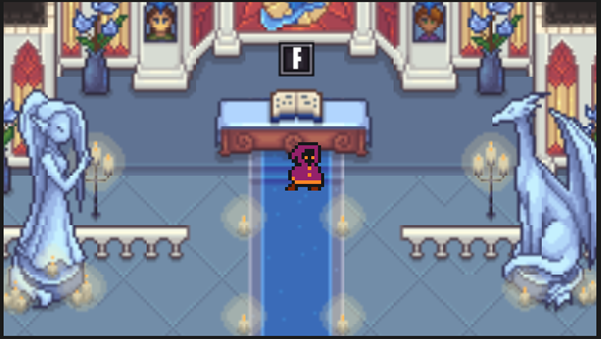
\includegraphics[scale=0.7]{Figure/mainscreen.png}
			\label{fig:main}
		\end{figure}
		\item Khu vực bên trong quyển sách nơi người chơi sẽ gặp npc hướng dẫn và tiếp nhận bài kiểm tra.
		\begin{figure}[H]
			\centering
			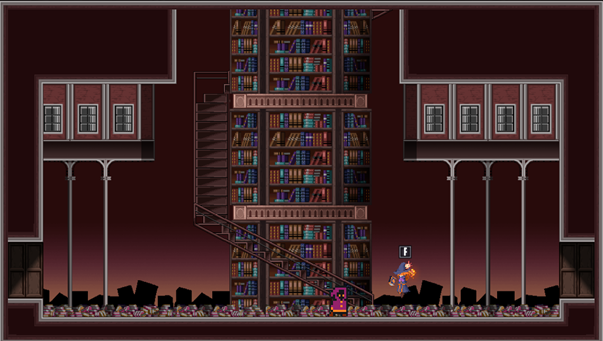
\includegraphics[scale=0.7]{Figure/library.png}
			\label{fig:library}
		\end{figure}
		\item Khu vực bên ngoài nhà thờ nơi đầy rẫy quái vật và người chơi phải tự mình khám phá.
		\begin{figure}[H]
			\centering
			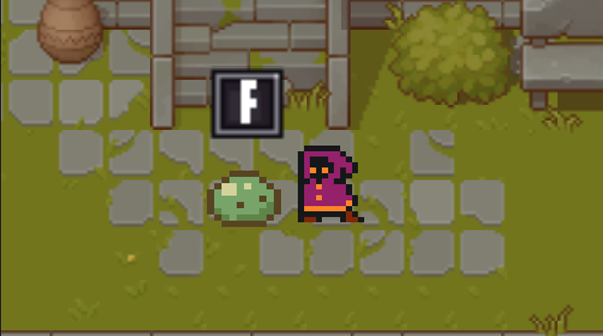
\includegraphics[scale=0.7]{Figure/interact.png}
			\label{fig:interact}
		\end{figure}
	\end{itemize}
	
	\item \textbf{Màn hình kiểm tra:} sau khi tương tác với npc hướng dẫn và màn hình kết quả sau một lần kiểm tra (cho biết trình độ người chơi):
	\begin{figure}[H]
		\centering
		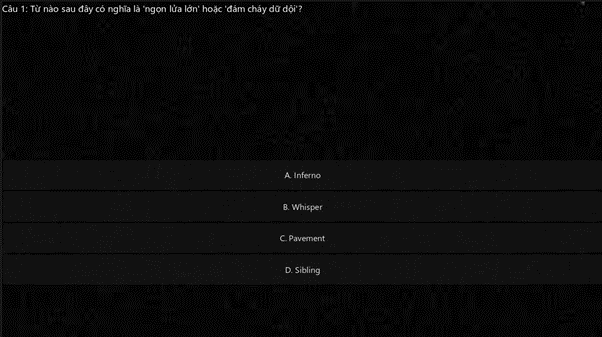
\includegraphics[scale=0.7]{Figure/ques.png}
		\label{fig:ques}
	\end{figure}
	
	\begin{figure}[H]
		\centering
		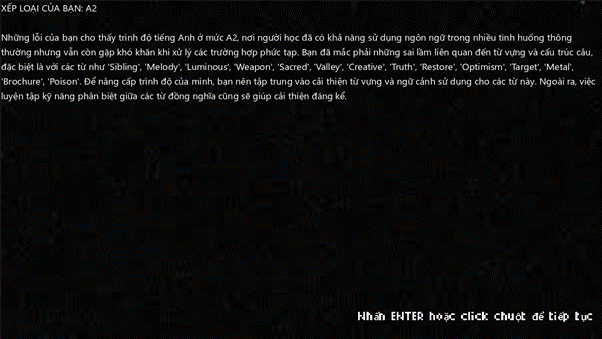
\includegraphics[scale=0.7]{Figure/tier.png}
		\label{fig:tier}
	\end{figure}
	
	\item \textbf{Màn hình chiến đấu:} Đây là màn hình có khá nhiều chi tiết, ở góc trên bên trái và phải lần lượt là số máu của người chơi và quái vật. Ở giữa phần máu sẽ là nơi hiển thị câu hỏi, cùng với các lựa chọn nằm ở phần giữa dưới cùng. Nếu trả lời sai thì sẽ xuất hiện pop up AI giải thích nằm giữa người chơi và quái vật.
	\begin{figure}[H]
		\centering
		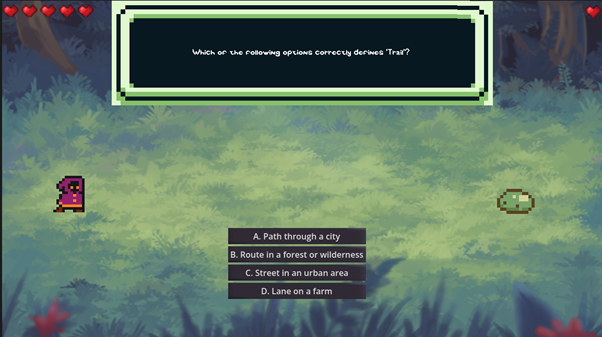
\includegraphics[scale=0.7]{Figure/combat1.png}
		\label{fig:combat1}
	\end{figure}
	
	\begin{figure}
		\centering
		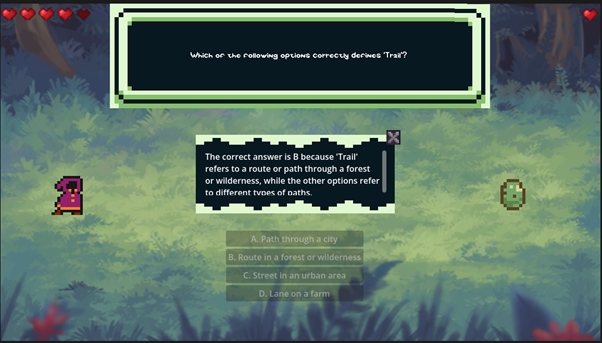
\includegraphics[scale=0.7]{Figure/combat2.png}
		\label{fig:combat2}
	\end{figure}
	
	\item Cuối cùng, chính là \textbf{màn hình kết quả trận đấu}: Màn hình này sẽ có 2 giao diện tùy theo kết quả là thua hay thắng.
	\begin{figure}[H]
		\centering
		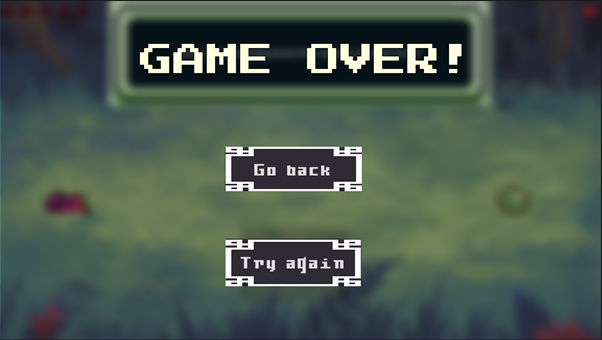
\includegraphics[scale=0.7]{Figure/gameover.png}
		\label{fig:over}
	\end{figure}
	
	\begin{figure}[H]
		\centering
		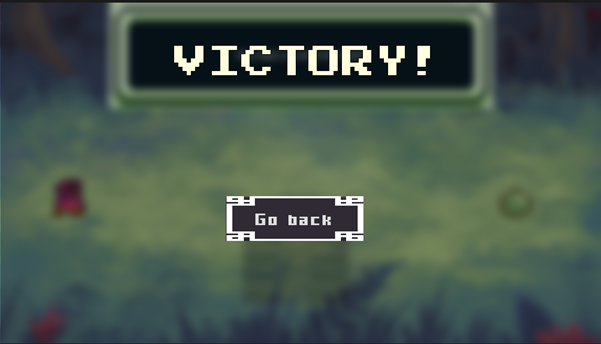
\includegraphics[scale=0.7]{Figure/victory.png}
		\label{fig:vic}
	\end{figure}
\end{itemize}

\subsubsection{Sơ đồ Figma}
\url{https://www.figma.com/design/HnMILOSGWcdUy0RT2fc36h/Untitled?node-id=0-1&t=i2gctwBXCzkZ9jcv-1}



